\documentclass[template.tex]{subfiles}

\usepackage{comment} 

\begin{document}

\begin{comment}
Andrew's comments: (THIS IS METHODS)
- describe modelling framework and details how you built everything
- now explain in detail what the package is \& can do, what the structure is like
- clarify that it is situated in complexity between custom scripts and modelling tools with graphical interfaces. It would be possible to design a graphical interface for this later on, but that is not the target audience.


"Python is a high-level programming language well suited to rapid development and prototyping, as well as being more accessible to domain scientists than low-level languages such as FORTRAN or C++." - Mobius GMD paper
- This is also due to the dynamic interpretation of python, which makes python slower, but python is rapidly developing and leveraging other lower level language for speed. Also has high functionality for parallelisation of code execution which is very relevant to complex marine ecosystem models. 

- clearly state limitations (scope) of phydra 
- mention that xarray-simlab is general enough to support IBMs! But not developed here.
\end{comment}



 %% \ SECTION 2
\section{The Phydra package: structure \& features} \label{Section:phydrapackage}
% 2nd Section:
% Background, theoretical framework. Specifics here!

Phydra is an open-source object-oriented Python package for modeling marine ecosystems, with to aim to support efficient, open and easily reproducible model development. 

In the current version Phydra includes a set of building blocks to create 0-dimensional ecosystem models of variable complexity. The building-blocks always refer to a process class, the modular unit of xarray-simlab model framework. A Phydra model instance would include the automatically added solving back end, as well as a model environment that collects certain forcings, multiple components (i.e. state variables) and fluxes acting on the components. Additional external parameters can be added to the model via forcing processes.

A typical model development workflow using Phydra would create a model instance from processes, then initialize this model with specific parameters and finally run the model to return the final output dataset. The model development is presented in further detail below.

The Phydra package is built on the wealth of functionality created by the open-source scientific Python community. The two packages xarray-simlab and GEKKO form the technical foundation of Phydra. Xarray-simlab provides the flexible model framework and GEKKO an efficient solver of large models. Below we describe how Phydra leverages these open-source projects to provide a tool-set to construct, modify, solve, analyse and share marine ecosystem models. 


\subsection{Python backend: xarray-simlab and GEKKO}

The library of modular processes and the user interface are based on the xarray-simlab package \citep{Bovy2018Xarray-simlab:Interactively}. 
Xarray-simlab provides a generic framework for building computational models in a modular fashion and an extension for model setup, running simulations and storing output using the xarray.Dataset structure. The Python package xarray provides an efficient and labelled multi-dimensional storage format, that is integrated with functionality for easy plotting, post-processing and storing of model output. Xarray.Datasets are easily converted to Netcdf files, a commonly used file format for biogeochemical data and large model output. 

In addition to a native storage solution, xarray-simlab provides the object-oriented framework for model building blocks, as well as the model setup and runtime user interface in Phydra. 
The building-blocks of the model are stored in decorated xarray-simlab process classes, which are slightly modified Python class structure. Within these process classes, all functions related to model formulation are stored. The Phydra library provides a set of basic components as well as base classes that can be modified by the user. At model initialisation the xarray-simlab framework automatically orders the processes according to their dependencies, and allows a model instance to be initialized with parameters and solved in a step-wise fashion. 

Xarray-simlab currently only provides step-wise simulation of model functions according to an explicit time step. Since such a solving routine is not ideal for complex systems of differential equations, we use the GEKKO Python package as a more robust back end to solving models built in Phydra. GEKKO is an open-source, object-oriented library of model construction, analysis and optimisation tools built on a core algebraic modelling language \citep{Beal2018GEKKOSuite}. Models can be constructed based on a common syntax and are compiled to efficient FORTRAN code before solving. 

When assembling a model in Phydra, there are certain basic processes that allow the GEKKO solver to assemble the full model. These are necessary so that each building block can communicate with the solver and are automatically included with every call to create a Phydra model.

Utilizing GEKKO as a backend solver within the xarray-simlab framework, we can combine the usability of a high-level language like Python with the efficient computation of lower-level languages. Additionally GEKKO provides a powerful interface to perform model optimisation, usage of which will be included with Phydra in future version. 

Both of these Python packages are relatively young and actively being developed, which provides some challenges but also allows for constant improvements to the functionality that Phydra provides.


\subsection{Phydra building-blocks}

Phydra provides a library of modular model building-blocks that can be used to assemble complex marine ecosystem models. The library is ordered into different logical components in a marine ecosystem, describing their function either as an environment, component, flux or forcing. 

The logic behind this order is that an ecosystem model would need at least one of each of these processes added in order to run. Phydra currently only supports running a single environment in a 0-dimensional setting with a flexible number of components and fluxes. In future versions the framework can potentially support multiple environments and dimensions.

The open-source code structure allows users to easy develop or modify processes to describe a specific ecosystem. The ordering of the building-blocks is not an implicit order, self-written building blocks can blur the boundaries and combine different functions.

The first version of the library will contain all processes needed to create the three model use cases presented in Section \ref{Section:UseCases}. Users of Phydra are very welcome to provide their own use cases to the standard library in a collaborative effort to support efficient, open and easily reproducible marine ecosystem model development.

These processes are classes that are provided with Phydra. We separate the processes into multiple logical categories that represent structures in a marine ecosystem model: Environments, Forcings, Components and Fluxes.

\subsubsection{Environments} \label{Section:PhysicalEnvironment}

A Phydra Environment defines the structure of the ecosystem and provides external inputs (i.e. forcings) that can be accessed by all processes linked to this environment. As a simple example we could take a chemostat model. The flow-through culture system is defined by a solution of nutrients that flows into a tank of fixed volume. Organisms within the tank grow, consume nutrients and are also flushed out of the system with the outflow of the medium. The Environment process in Phydra describing a chemostat would have the nutrient concentration in the medium, as well as the flow-rate of the system as required external forcing processes. The forcing input can be supplied from different Forcing processes, for example with a time-varying flow rate. Components, which define the state variables in our model, are grouped within our chemostat Environment and the Fluxes (e.g. nutrient uptake or mortality) affect Components within this Environment. We can add any number of Components from the Phydra library into our Environment and between the Components we could add any number of interactions.

Phydra as of now provides an easily modifiable base environment and implementations of a chemostat environment, as well as a slab-ocean environment. The first release of Phydra supports only single 0-dimensional implementations of these basic ecosystem models, but extending this to 2- and 3-dimensional flexibility is a high development priority. 

\subsubsection{Forcings} \label{Section:ForcingSection}

Forcings are defined as providing an external constant or time-varying parameter to the model. These parameters can be used in fluxes that reference the forcing type, but are most often used in conjunction with an environment that takes the specific type of forcing as an input. Included with this version of Phydra we have the necessary forcing types that have to be supplied to the provided environments. For a chemostat model, this is a source concentration of a component in the medium, as well as a flow rate of the system. The slab-ocean Environment interfaces with forcings describing the concentration of a component below the mixed layer, movement of the mixed layer depth (MLD), irradiance at surface and temperature within the mixed layer. There are basic methods supplied to create either constant forcing or values over time based on mathematical functions. Additionally a base forcing can be modified by a user to provide any external data, which can then be used by other processes in the library. The flexible class-based structure allows a process inheriting from the base MLD forcing process to be recognised as an MLD forcing in the fluxes and processes of our model.

\subsubsection{Components}

An ecosystem model tracks chemical compounds as well as organisms via state variables. These state variables can define completely different components of a model, or represent a functional group. Components within Phydra are defined at this higher level and can contain a single state variable or an array of state variables that share common fluxes with differing parameterisation. Each component is added to the model with a specific label that is used to reference this component in all processes affecting or dependent on it. The actual dimensions of a model component are initialized after passing a parameter at model setup. This has been designed for easily testing different levels of ecosystem complexity. As shown in the second use case, where this is useful is in setting up phytoplankton size classes in trait-based models. All phytoplankton state variables grow on a common nutrient, but uptake parameters are related to allometries of cell size. A phytoplankton component could be initialized, with a certain size range and number of state variables. Within the allometric growth process parameters are dynamically initialized based on the size provided by the component. 
In addition to size, the component could be modified to include information on units or other specific parameters relevant to the model. The added flexible dimensionality of components was designed with the current issues in marine ecosystem model in mind. The effects of different levels of complexity, in the number and definition of phytoplankton functional types (PFT) for example, is not routinely tested in marine ecosystem models. Phydra provides a framework that allows for easy testing through flexible modification of such model complexity at model setup.



\subsubsection{Fluxes}
The previous building blocks of an environment, components and forcing create the structure of the model, but when solved at this stage there would be no meaningful simulation. In order to define exchanges of matter between components flux processes are added to our model instance, defining the affected components via labels at model setup.
There are multiple types of fluxes provided as base classes in the library. These base classes are defined by the type of interaction between components. Single fluxes provide loss or gain processes to a single variable, such as sinking or influx from outside the ecosystem. In order to simplify creating common forcing fluxes, a single flux process can take list of affected components as input at model setup. An example for more complex flux type are exchange fluxes, where a flux affects one component as a source and another as a sink. These can be set up with flexible dimensionality of components. Grazing fluxes are a slightly more complicated subclass of a grid-wise flux, as ingestion is usually normalized by total prey availability, so all forcing interactions need to be calculated in a dynamically generated matrix of all prey items consumed by a component.

The calculation of a primary producers growth rate is usually one of the more complex fluxes in a marine ecosystem, perhaps second to grazing formulations. In the most simple case the growth of phytoplankton in our slab model would be an exchange flux from the component that grows, dependent on a saturating Monod (or Michealis-Menten) function of a resource concentration. There is no distinction between the rate of nutrient uptake and the assimilation of these nutrients. We can add this simplified relationship to our model using the MonodGrowth process, which is applied in our second use case. At model setup the user only needs to provide the label of the resource that is consumed and the component that is growing, in addition to parameters such as the half-saturation constant for uptake, to have this growth function implemented.
More complex representations of growth in marine ecosystem models track additional factors limiting growth. In our first use case, phytoplankton growth is limited by nutrient uptake, according to Monod, as well as temperature and light-availability in the mixed layer. These additional growth limiting factors are included in the library as a MonodLightTempGrowth process, that inherits the forcing for average temperature in the mixed layer and PAR at surface from the slab environment.




\subsection{Model development workflow}

Phydra is a tool-box for marine ecosystem modeling, that is freely extensible by a user to be applied to many different use cases. Our goal is to make the technical implementation of writing functions and setting up a model more accessible, so that the focus can be on creating the most appropriate model structure and parameterisation for the specific scientific hypothesis that is being investigated. 
Phydra is by nature a collaborative project that encourages sharing and modification of ecosystem models.

Constructing marine ecosystem models in Phydra is by nature flexible, but the user can follow a general workflow of assembling models from the library of processes. This workflow is visualized in \ref{Figure:phydraschematics} and will be further explained below.

\subsubsection{Installing and running Phydra}
The Phydra package is available via the Python pip package manager, but we encourage using Conda as a package manager that is provided with the scientific Anaconda Python distribution.
Please follow the up-to-date instructions on the Github repository for installation of Phydra and its dependencies.
% CONDA NAME DROP
Since python is a fast developing language, we will provide instructions to install a fully compatible virtual environment with the Conda package manager separate from a users standard python environment. For interactive coding and prototyping of models using Phydra, we recommend using the Jupyter environment that is available via Conda. For more complex and larger model runs on servers or clusters python scripts are preferable.


\subsubsection{Model creation}

To create a Phydra model object, the desired environment, forcings, components and fluxes are provided with their corresponding label to the \texttt{phydra.Model()} function.

Ideally the model can be assembled from processes already provided in the Phydra library. The framework allows most processes that are not included to be included as modifications of provided base classes or custom written processes. 

At model initialisation the processes to be included are added to the model with a label specified by the user. These labels will be the specific name of the process in this model instance. At model creation, the labels are used to reference a process and provide necessary parameters.
The xarray-simlab framework automatically checks that all references between processes are fulfilled and orders the processes in their logical order. 
Finally the call \texttt{phydra.Model()} returns a Phydra model object. This model object contains all processes in the model and allows the user to view all parameters required as input at model setup. 

\subsubsection{Model setup}

An Phydra model object is itself only a collection of abstract processes, that defines the parameters needed at model setup. The next step towards computation is to embed this model in our xarray.Dataset storage at the given dimensionality and with the given parameters.

This is done using the \texttt{phydra.create\_setup()} function. The necessary arguments are values for all input parameters as well as the required model output. 

The function returns a labeled xarray dataset, that contains the model backend.


Input parameters can have a required dimensionality, 

The model output can be modified according to the question at hand. For large functional group models, it would make sense to store the output of each component indidividually, while a simple NPZD model can best be visualized by returned all components along a shared dimension.
can be returned for all state variables initialized in the environment
or grouped per specific component


it is easy to add smaller modifications after this stage, by updating the model 
test different dimensionality in a structured manner
you can update parameters and create a new initialized model setup from an existing one

\subsubsection{Runtime}
% -> model_instance.xsimlab.run()
% relatively straightforward, this will first initialize the model data variables according to the added processes and parameters supplied, and then start model evaluation

you can also create a batch dimension for a specific parameter, that you specify at model runtime and the model is executed for every 

- explain what the options are to run the model, depends on if a time implicit method will be added to solve, or if it will just remain with the time explicit steps of xarray-simlab

% model execution in parallel currently only works along batch dimensions,
% both xarray-simlab and GEKKO provide parallelization functionality future versions of phydra could leverage to run large models more efficiently. 


\subsubsection{Model Diagnostics and additional functionality}

If the option is specified at setup, the model output will include not just the state variables, but the values of all fluxes.

\textit{NOTE: there are a few possible addons that might very well be included in the first version, depending on development progress. I will keep them as bullte points below.}

- Gekko provides functionality to view the assembled model as latex output

- Model optimisation (i.e. parameter fitting) is well supported by the GEKKO backend provided with phydra. 


\subsubsection{Modification and further development}

- Similar to how a forcing process can easily be subclassed to supply a different forcing, other processes in xsimlab can be easily subclassed and modified to have a different function, as long as the interaction between state variables matches
- Explain interface to process subclasses, and how it is relatively easy to set up xsimlab processes with slightly different  formulations, but the same basic interaction


% OPEN SOURCE CONTRIBUTION 
Phydra (like Xarray-simlab and GEKKO) is an open-source project. Contributions are welcome and in fact greatly appreciated. Users can contribute in many ways by reporting bugs, submitting feedback, contributing to the development of the code or the documentation. Please read the contributing guidelines on the Github repository for further details.






%%% TWO-COLUMN FIGURES
%
%%f
\begin{figure*}[t]
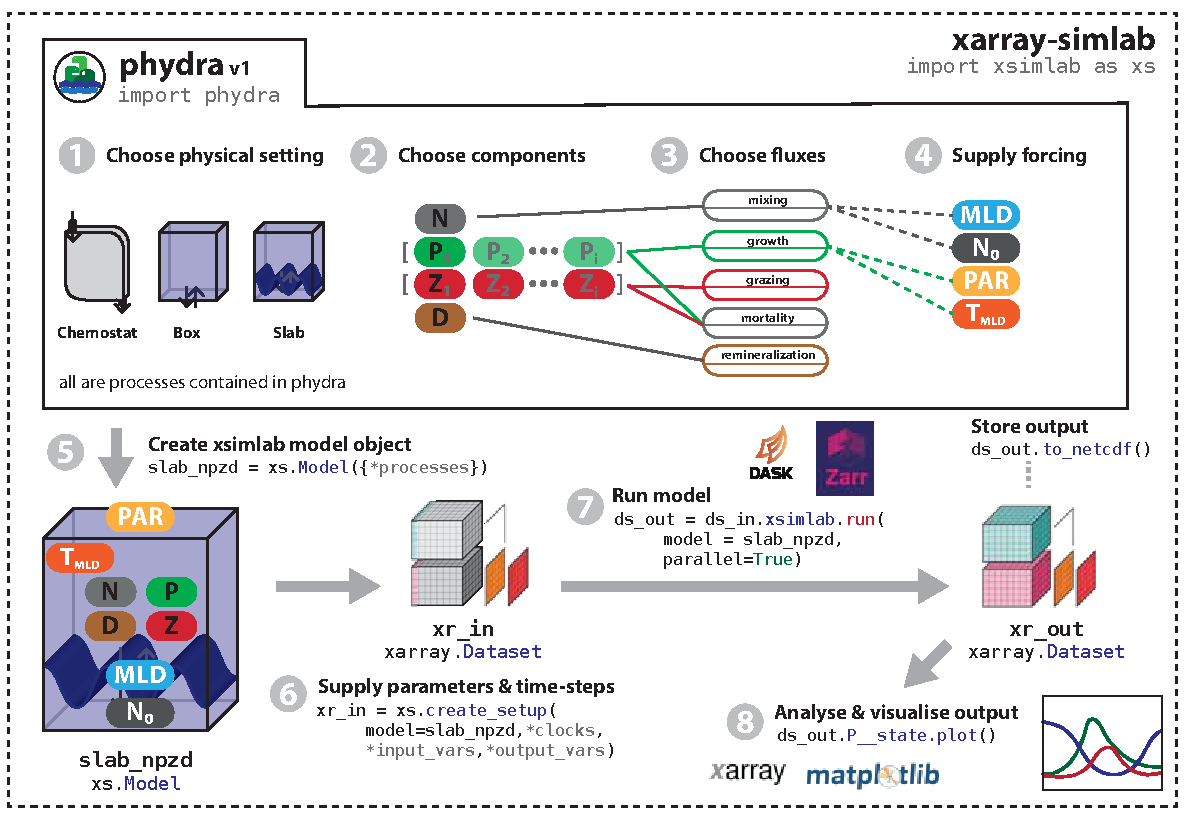
\includegraphics[width=12cm]{Figures/firstdraft_schematics/01__schematics_phydra_1.pdf}
\caption{The phydra package is embedded within the xarray-simlab framework. phydra contains a library of physical settings (1), components (i.e. state variables) (2), fluxes (3) and forcing variables (4), that can be combined and reused to create an xarray-simlab model instance. Xarray-simlab provides the functionality to define the model (5) from processes in the phydra library, supply parameters and create an xarray input (6), then run the model (7) and the resulting output is dynamically stored in another xarray, with fully labelled dimensions and containing all parameters.}
\label{Figure:phydraschematics}
\end{figure*}





% Everything below here is optional, it depends on what I can actually do in the package
% this is a custom function to be able to see references when rendering subfiles:
\biblio

\end{document}